\chapter{Perancangan Perangkat Lunak}
\label{chap:perancangan perangkat lunak}

Pada bab ini akan dibahas mengenai perancangan aplikasi untuk membuat \textit{Twitter bot} untuk mencari jalur transportasi publik sesuai analisa yang sudah dibahas pada bab 3.

\section{Perancangan Kelas}
Sub bab ini akan membahas tentang rancangan kelas dan \textit{method} yang akan dibuat pada perangkat lunak \textit{Twitter bot} untuk mencari jalur transportasi publik. Untuk lebih jelas mengenai kelas yang ada pada aplikasi ini, penulis menyajikan gambar kelas diagram yang dapat dilihat pada Gambar~\ref{fig:classDiagramSkripsi}

\begin{figure}[htbp]
	\centering
		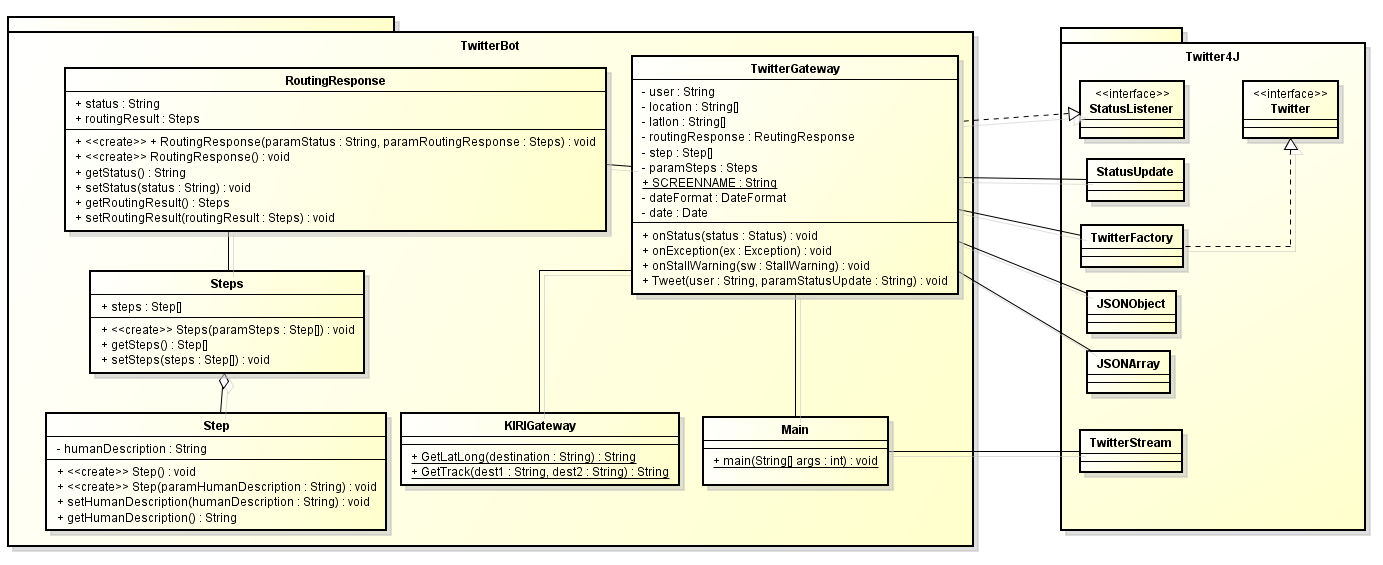
\includegraphics[width=1.00\textwidth]{C:/Skripsi/doc/DokumenSkripsi/Gambar/classDiagramSkripsi.PNG}
	\caption{Diagram Kelas Pembuatan \textit{Twitter bot} untuk Mencari Jalur Transportasi Publik}
	\label{fig:classDiagramSkripsi}
\end{figure}


\begin{itemize}
		\item Kelas Main merupakan kelas yang berfungsi untuk membuat koneksi dengan Twitter ketika perangkat lunak dijalankan.
		
				\begin{itemize}
							\item Method
							
									\begin{itemize}
												\item public static void main(String[] args), merupakan method main untuk menjalankan program.
										
									\end{itemize}
				\end{itemize}
		
		\item Kelas Twitter Gateway, merupakan kelas untuk menangkap dan membalas \textit{tweet}. Kelas Twitter Gateway ini mengimplementasikan \textit{StatusListener}.
		
		
				\begin{itemize}
							\item Atribut
							
							
									\begin{itemize}
												\item String user, digunakan untuk menampung nama akun pengguna \textit{Twitter bot}.
												\item String location[], berupa \textit{array} yang digunakan untuk menampung lokasi awal dan lokasi tujuan.
												\item String latlon[], berupa \textit{array} yang digunakan untuk menampung koordinat lokasi awal dan koordinat lokasi tujuan.
												\item RoutingResponse routingResponse, merupakan atribut yang digunakan untuk menampung hasil yang diberikan oleh KIRI API.
												\item Step[] step, berupa \textit{array} yang berguna untuk menampung langkah-langkah informasi perjalanan.
												\item Steps steps, merupakan atribut yang berguna untuk menampung semua step.
									\end{itemize}
							
							\item Method
							
									\begin{itemize}
												\item public void onStatus(Status status), merupakan \textit{method} yang berguna untuk menangkap \textit{tweet} dan memproses \textit{tweet} tersebut. Jika ada \textit{tweet} yang di-\textit{mention} kepada akun \textit{Twitter bot} dan \textit{tweet} yang diterima merupakan \textit{tweet} untuk mencari jalur transportasi publik, maka \textit{tweet} tersebut akan dimasukan ke atribut yang sudah disediakan. Atribut tersebut antara lain adalah \textit{user}, lokasi awal dan lokasi tujuan. Setelah mendapatkan lokasi awal dan lokasi tujuan barulah proses pencarian dimulai dengan menggunakan \textit{GetLatLong method} dan \textit{GetTrack method} yang terdapat di kelas KIRIGateway. Hasil pencarian akan dimasukan ke dalam atribut \textit{routingResponse}, \textit{step}, dan \textit{steps}. Setelah itu akan dilakukan pemanggilan \textit{Tweet method} untuk melakukan proses \textit{reply}.
												\item public void onDeletionNotice(StatusDeletionNotice statusDeletionNotice), merupakan \textit{overload method} dari kelas \textit{interface} \textit{StatusListener}.
												\item public void onTrackLimitationNotice(int numberOfLimitedStatuses), merupakan \textit{overload method} dari kelas \textit{interface} \textit{StatusListener}.
												\item public void onScrubGeo(long userId, long upToStatusId), merupakan \textit{overload method} dari kelas \textit{interface} \textit{StatusListener}.
												\item public void onException(Exception ex), merupakan \textit{method} yang berguna untuk menangkap \textit{exception}.
												\item public void onStallWarning(StallWarning sw), merupakan \textit{overload method} dari kelas \textit{interface} \textit{StatusListener}.
												\item public void Tweet(String user, String paramStatusUpdate), merupakan \textit{method} untuk melakukan \textit{reply} yang ditujukan kepada akun pengguna \textit{Twitter bot}. Twitter hanya dapat melakukan \textit{tweet} dengan batas 140 karakter, oleh karena itu \textit{method} ini akan mengatasi keterbatasan \textit{tweet} tersebut dengan melakukan pembagian \textit{tweet}. Method ini akan memberi tambahan waktu yang sesuai dengan \textit{server} di setiap akhir \textit{tweet}, hal ini bertujuan untuk menghindari adanya \textit{duplicate tweet}.
									\end{itemize}
				\end{itemize}
		
		\item Kelas KIRIGateway merupakan kelas untuk memanggil KIRI API. Pemanggilan KIRI API ini digunakan untuk mendapatkan koordinat suatu lokasi dan mencari jalur transportasi publik.
		
		
				\begin{itemize}
							\item Method
							
							
									\begin{itemize}
												\item public static String GetLatLong(String destination), merupakan \textit{method} yang digunakan untuk mencari koordinat dari suatu lokasi. Hasil kembalian dari \textit{method} ini berupa \textit{latitude} and \textit{longitude} yang diberikan oleh KIRI API lalu diubah ke dalam bentuk \textit{String}.
												\item public static String GetTrack(String dest1, String dest2), merupakan \textit{method} yang digunakan untuk mencari jalur transportasi publik dari lokasi awal ke lokasi tujuan. Hasil kembalian dari \textit{method} ini adalah langkah-langkah perjalanan dari lokasi awal ke lokasi tujuan dengan menggunakan transportasi publik.
									\end{itemize}
				\end{itemize}
		
		
		\item Kelas RoutingResult merupakan kelas untuk menampung hasil kembalian dari KIRI API
		
		
				\begin{itemize}
							\item Atribut
					
					
									\begin{itemize}
												\item status, merupakan atribut yang digunakan untuk menyimpan status dari hasil pencarian.
												\item routingResult, merupakan atribut yang digunakan untuk menyimpan langkah-langkah perjalanan.
									\end{itemize}
					
							\item Method
					
					
									\begin{itemize}
												\item public RoutingResponse(String paramStatus, Steps paramRoutingResult), merupakan \textit{constructor} dari kelas RoutingResult.
												\item public RoutingResponse(), merupakan \textit{constructor} dari kelas RoutingResult.
												\item public String getStatus(), merupakan \textit{getter} dari atribut status.
												\item public void setStatus(String status), merupakan \textit{setter} dari atribut status.
												\item public Steps getRoutingResult(), merupakan \textit{getter} dari atribut routingResult.
												\item public void setRoutingResult(Steps routingResult), merupakan \textit{setter} dari atribut routingResult.
									\end{itemize}
				\end{itemize}
		
		\item Kelas Step merupakan kelas untuk menampung jalur perjalanan dari lokasi awal ke lokasi tujuan dengan menggunakan transportasi publik yang diberikan oleh KIRI API.
		
		
				\begin{itemize}
							\item Atribut
					
					
									\begin{itemize}
												\item String humanDescription, merupakan atribut untuk menjelaskan cara perjalanan yang bahasanya dimengerti oleh pengguna.
									\end{itemize}
					
							\item Method
					
					
									\begin{itemize}
												\item public Step(), merupakan \textit{constructor} dari kelas Step.
												\item public Step(String paramHumanDescription), merupakan \textit{constructor} dari kelas Step.
												\item public String getHumanDescription(), merupakan \textit{getter} dari atribut humanDescription.
												\item public void setHumanDescription(String humanDescription), merupakan \textit{setter} dari atribut humanDescription.
									\end{itemize}
				\end{itemize}
		
		\item Kelas Steps merupakan kelas untuk menampung kumpulan step.
		
		
				\begin{itemize}
							\item Atribut
					
					
									\begin{itemize}
												\item Step[] steps, merupakan atribut yang berisi \textit{array} step
									\end{itemize}
					
							\item Method
					
					
									\begin{itemize}
												\item public Steps(Step[] paramSteps), merupakan konstruktor dari kelas Steps.
												\item public Step[] getSteps(), merupakan \textit{getter} dari atribut steps.
												\item public void setSteps(Step[] steps), merupakan \textit{setter} dari atribut steps.
									\end{itemize}
				\end{itemize}
\end{itemize}


\section{Sequence Diagram}
Pada sub bab ini, akan dijelaskan alur program dengan menggunakan \textit{sequence diagram} pada Gambar~\ref{fig:Sequence Diagram Final}

\begin{sidewaysfigure}[htbp]
	\centering
		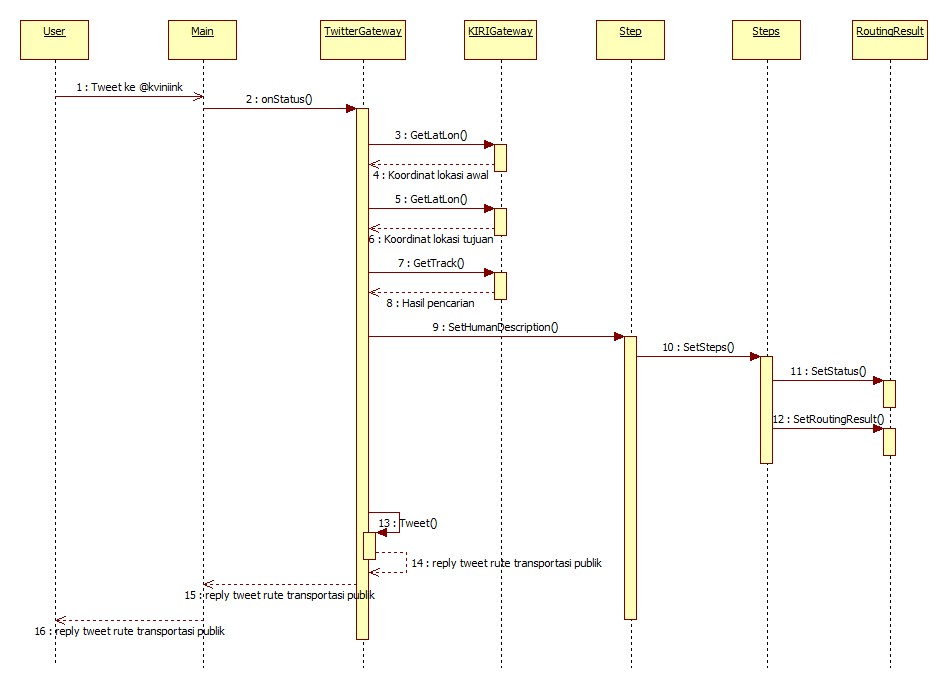
\includegraphics[width=1.00\textwidth]{C:/Skripsi/doc/DokumenSkripsi/Gambar/Sequence Diagram Final.jpg}
	\caption{Sequence Diagram \textit{Twitter bot} untuk Mencari Jalur Transportasi Publik}
	\label{fig:Sequence Diagram Final}
\end{sidewaysfigure}


Pertama, perangkat lunak akan melakukan \textit{streaming} pada saat kelas \textit{main} dijalankan. Kelas \textit{main} akan membuka gerbang untuk mengakses \textit{Twitter API}, dengan menggunakan \textit{Streaming} API perangkat lunak akan menangkap semua \textit{tweet} yang melakukan \textit{mention} kepada akun \textit{Twitter bot} @kviniink. Perangkat lunak akan terus melakukan \textit{streaming tweet} hingga perangkat lunak dinon-aktifkan.

Kelas TwitterGateway akan memproses \textit{tweet} yang di-\textit{mention} kepada akun \textit{Twitter bot} @kviniink. \textit{onStatus Method} akan melakukan pengecekan apakah \textit{tweet} tersebut merupakan \textit{tweet} untuk mencari jalur transportasi publik atau bukan. Jika benar, maka nama akun pengirim, lokasi awal, dan lokasi tujuan akan disimpan di atribut yang sudah disediakan. Setelah itu akan dicari koordinat dari masing-masing lokasi menggunakan KIRI API. Proses pencariian koordinat dilakukan oleh kelas KIRIGateway.

Kelas KIRIGateway akan memanggil \textit{GetLatLon method} untuk mencari koordinat suatu lokasi. Setelah didapatkan koordinat lokasi awal dan lokasi tujuan, kelas TwitterGateway akan mengubah hasil dari \textit{GetLatLon method} yang berupa \textit{JSON} menjadi format \textit{String}. Setelah didapatkan koordinat lokasi awal dan koordinat lokasi tujuan maka hasil dari masing-masing koordinat dikembalikan kepada kelas KIRIGateway untuk dicari jalur transportasi publik dari lokasi awal menuju lokasi tujuan menggunakan \textit{GetTrack method}. Hasil dari \textit{GetTrack method} akan disimpan pada atribut \textit{step, steps}, dan \textit{routingResult}. \textit{Method setHumanDescription} berguna untuk menyimpan hasil kembalian KIRI pada atribut \textit{step}. \textit{Method setSteps} merupakan \textit{method} untuk menyimpan \textit{step} kedalam atribut \textit{steps}. \textit{Method setStatus} merupakan \textit{method} untuk menyimpan \textit{status} hasil kembalian KIRI kedalam atribut \textit{status}. \textit{Method setRoutingResult} merupakan \textit{method} untuk menyimpan \textit{steps} kedalam atribut \textit{routingResult}.

Setelah selesai, langkah-langkah jalur transportasi publik siap untuk di \textit{reply} kepada pengguna. Proses \textit{reply} dilakukan oleh \textit{tweet method} yang terdapat pada kelas TwitterGateway. \textit{Tweet} tersebut berisi tentang jalur transportasi publik dari lokasi awal menuju lokasi tujuan.\textit{Tweet} akan di-\textit{reply} satu per satu sesuai dengan banyaknya \textit{step} yang ada. Perangkat lunak akan terus melakukan proses tersebut hingga perangkat lunak dinon-aktifkan.

\newpage
\section{Perancangan Antarmuka}
Perangkat lunak yang dibangun memiliki antarmuka berbasis teks. Untuk menjalankan perangkat lunak \textit{Twitter bot} cukup dengan menjalankan aplikasi. \textit{Twitter bot} akan terus berjalan hingga perangkat lunak di \textit{non}-aktifkan. Antarmuka yang akan digunakan oleh pengguna menggunakan antar muka yang disediakan oleh Twitter. Antarmuka yang disediakan oleh Twitter adalah antarmuka yang terdapat pada:
\begin{enumerate}
	\item \textit{website} Twitter,
	\item Android,
	\item iOS,
	\item Windows Phone.
\end{enumerate}

%\section{Perancangan Antar Muka}
%Perangkat lunak yang akan dibangun memiliki antar muka berbasis teks, tetapi tampilan antar muka untuk pengguna berbeda-beda. Interaksi dengan pengguna dapat dilakukan melalui \textit{website} atau aplikasi Twitter.


%Gambar ~\ref{fig:Homepage Mobile Twitter} adalah tampilan antar muka dari Twitter yang diakses melalui \textit{website mobile} Twitter \url{https://mobile.twitter.com/}. Antar muka \textit{Twitter bot} akan menampilkan \textit{tweet} yang diterima oleh perangkat lunak, dan menampilkan hasil \textit{tweet} yang di-\textit{reply} \textit{Twitter bot} kepada pengguna.

%\begin{figure}[htbp]
%	\centering
%		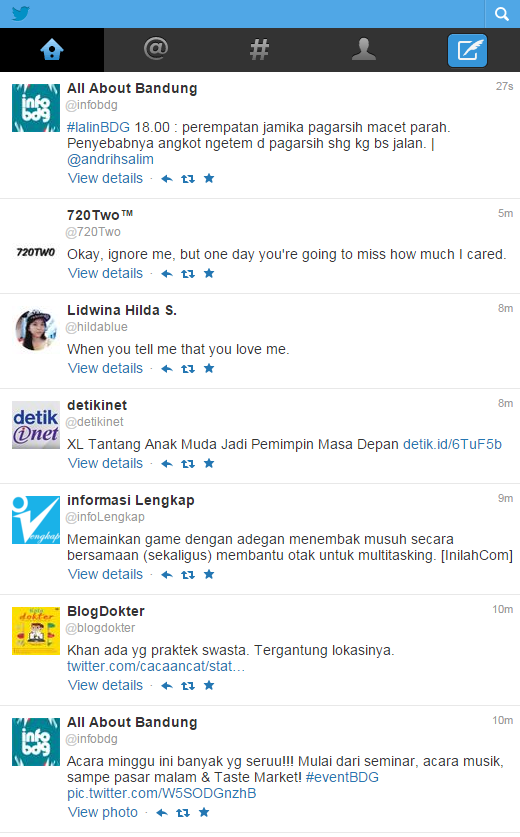
\includegraphics[width=0.75\textwidth]{C:/Skripsi/doc/DokumenSkripsi/Gambar/Homepage Mobile Twitter.PNG}
%	\caption{Homepage Twitter yang Diakses Melalui Mobile Twitter}
%	\label{fig:Homepage Mobile Twitter}
%\end{figure}


